\newpage
\section{Method} \label{sec:method}
\subsection{Setup}
\subsection{Data Set}

\newpage
\subsection{Curve Fit}
\label{sec:fit}
The peaks were fit to the data with \texttt{scipy.optimize.curve\_fit}\cite{scipy} using a {\scshape Gaussian} peak given in \eqref{eq:gauss}
\begin{align}
    f(x) = A\cdot e^{-\frac{(x-\mu)^2}{2\sigma^2}} \label{eq:gauss}
\end{align}
For Xenon the peaks at $m=132$ amu and $m=131$ amu and $m=129$ overlap, thus a superposition of three {\scshape Gaussians} separated by $\Delta m_1 = 1$ amu and $\Delta m_2 = 3$ amu was used to fit the peaks, this equation is given in \eqref{eq:gaussxe}.
\begin{align}
    f(x) = A_1\cdot e^{-\frac{(x-\mu)^2}{2\sigma_1^2}} + A_2\cdot e^{-\frac{(x-\mu - 1)^2}{2\sigma_2^2}} + A_3\cdot e^{-\frac{(x-\mu-3)^2}{2\sigma_3^2}} \label{eq:gaussxe}
\end{align}
The fit-function also provides us with the covariance-matrix for the parameters.
An example is shown in figure \ref{fig:gauss_int}. In order to get the amount of the measured compound we have to calculate the area of the fit. If we just summed up the bins from $\mu-3\sigma$ to $\mu+3\sigma$, but then we also include the noise. The area can directly be calculated from the {\scshape Gaussian} as given in \eqref{eq:gauss_int}.
\begin{align}
    \int_{-\infty}^{+\infty} A\cdot e^{-\frac{(x-\mu)^2}{2\sigma^2}} \mathrm{d}x = \sqrt{2\pi}A\sigma \label{eq:gauss_int} 
\end{align}
\begin{figure}[h!]
    \centering
    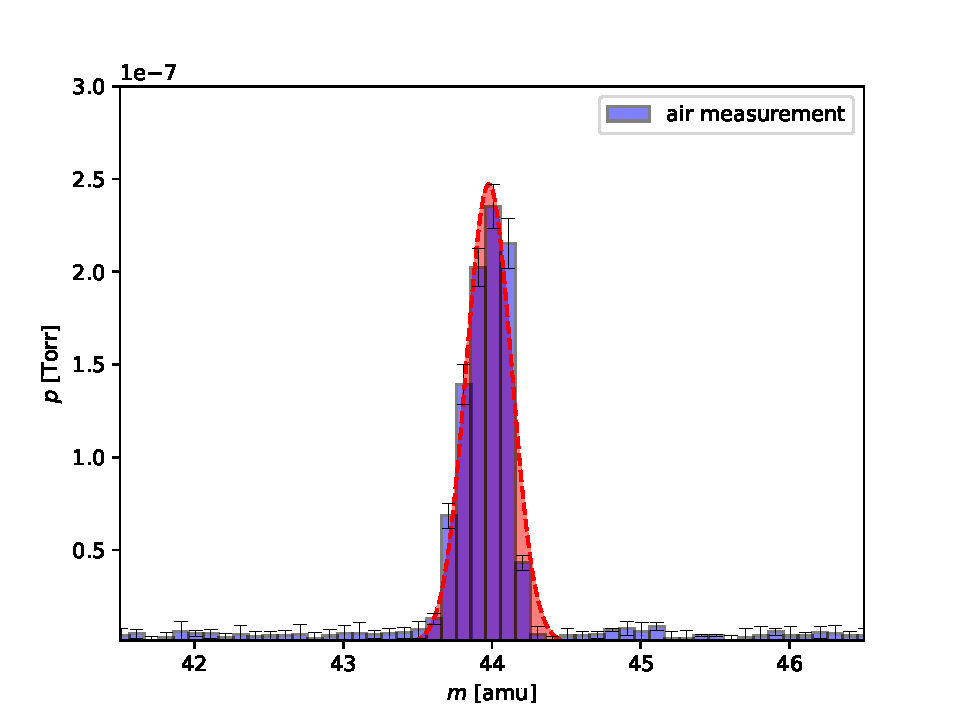
\includegraphics[width=\textwidth]{Report/DataResultsPlots/peak.pdf}
    \caption{An example of our fit applied to a data-set gathered during this experiment.}
    \label{fig:gauss_int}
\end{figure}


\subsection{Calibration}
Upon looking at the fit Peaks for Argon and Xenon, we noticed that there was a slight deviation from the expected values. We thus had to calibrate the measurement of the detector with this two data-sets. Equation \eqref{eq:calibrate} was applied to all gathered data in order to calibrate the $m$ axis.
\begin{align}
    m \to m_\text{Ag, true} + \frac{m_\text{Xe, true} - m_\text{Ag, true}}{m_\text{Xe, fit} - m_\text{Ag, fit}} \cdot (m - m_\text{Ag, fit}) \label{eq:calibrate}
\end{align}
Where $m_{i, \text{true}}$ are taken from literature and $m_{i, \text{fit}}$ are obtained from our fit.
The error on this calibration is derived in \ref{app:err_cal}.
\subsection{Error Estimation}


